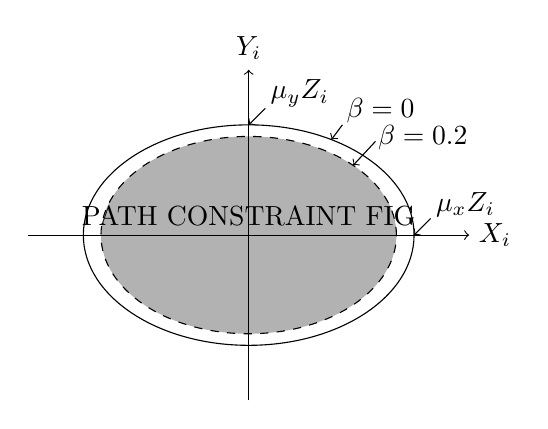
\begin{tikzpicture}[scale = .7]
	% Parameters
	\def\outerX{3}   % x radius of outer ellipse
	\def\outerY{2}   % y radius of outer ellipse
	\def\gap{0.2}    % distance between outer and inner ellipse
	\def\innerX{2.68}
	\def\innerY{1.79}
	
	% Draw outer ellipse
	\draw[] (0,0) ellipse [x radius=\outerX, y radius=\outerY];
	
	% Draw inner ellipse filled with color
	\fill[black!30] (0,0) ellipse [
	x radius={\innerX},
	y radius={\innerY}
	];
	\node[above] at (0,0) {PATH CONSTRAINT FIG};
	\draw[dashed] (0,0) ellipse [
	x radius={\innerX},
	y radius={\innerY}
	];
	
	% Draw axes
	\draw[->] (-\outerX-1,0) -- (\outerX+1,0) node[right] {$X_i$};
	\draw[->] (0,-\outerY-1) -- (0,\outerY+1) node[above] {$Y_i$};
	
	% Arrows pointing to the ellipses
	\draw[->,thin] (1.7,2) -- ({\outerX*cos(60)},{\outerY*sin(60)}) node[midway, above right] {$\beta=0$};
	\draw[->,thin] (2.3,1.7) -- ({(\innerX)*cos(45)},{(\innerY)*sin(45)}) node[midway, right, shift={(0.05,.2)}] {$\beta=\gap$};
	
	% Arrows pointing to the ellipses
	\draw[->,thin] ({\outerX+.3},.3) -- (\outerX,0) node[midway, above right,shift={(.05,0)}] {$\mu_x Z_i$};
	\draw[->,thin] (.3,{\outerY+.3}) -- (0,\outerY) node[midway, above right,shift={(.05,0)}] {$\mu_y Z_i$};
	
\end{tikzpicture}